% LREC-COLING 2024 Example; 
% LREC Is now using templates similar to the ACL ones. 
\documentclass[10pt, a4paper]{article}
\usepackage[review]{lrec-coling2024} % this is the new style
\title{Can The Potential for Offline Harm Events in Social Media Texts Be Identified Without knowing the Context ?}
\name{Ram Mohan Rao Kadiyala} 
\address{   University of Maryland , College Park\\
            rkadiyal@terpmail.umd.edu\\}
\abstract{
This paper explores the capability to assess the potential for offline harm events posed by online social media texts without contextual knowledge. Engaging in the TRAC-2024 shared task : Offline Harm Potential Identification (HarmPot-ID), we investigate a vital classification challenge: determining a post's likelihood to incite offline harm, such as protests, clashes or riots and identifying the target groups(s). Our analysis encompasses two main tasks: the prediction of offline harm potential across four categories, ranging from no risk to certainty of causing harm, and identifying the probable target(s) of such harm among five broad groups including gender, religion, caste, descent and political ideology. Leveraging a dataset comprising of 4 languages - English and code-mixed Hindi, Bangla, Manipuri texts from platforms like YouTube, Twitter, Telegram, etc.., we apply and evaluate various computational approaches, including transformer models, Large language models and a keyword-based filtering strategy. Our findings offer insights into the effectiveness of these methods in identifying harmful content without context, suggesting avenues for practical applications in monitoring and mitigating online threats. The paper also discusses the strengths and weaknesses of each of the approaches and methods.
 \\ \newline \Keywords{Social Media Analytics, Hate Speech Recognition, Text Classification} }
\begin{document}
\maketitleabstract
\section{Introduction}
\label{sec:intro}
With an overwhelming amount of content being shared daily on various social media platforms by numerous users, identifying posts that have the potential to incite offline harm, such as riots, protests, or clashes, becomes a significant challenge. The complexity of this task is compounded by the diversity of the content, ranging from text in multiple languages to coded and code-mixed messages. This paper delves into two specific tasks within this context. The first task is classifying the text based on the likelihood of inciting  offline harm events among 4 classes on a scale of 0 to 3. The second task involves binary classification among 5 categories about what group is likely being targeted by the text : gender, religion, descent, caste, political ideology. We have tested various approaches and methods including keyword based filtering, transformers, LLMs towards improving classification using micro f1 score as primary metric for both the subtasks along with recall.

\section{Dataset}
\label{sec:dataset}

The dataset \citep{kumar2024harmpot} used in this study is detailed in three tables, providing an extensive breakdown of the collected social media posts. The texts range from single word to multiple sentences , sometimes just emojis with no text consisting on 4 languages : English(en) , code-mixed and direct versions of Bengali(bn), Meitei(mni), Hindi(hi). \autoref{table:1} shows the distribution of labels for the potential offline harm (subtask 1A) across the training, development, and test datasets. The distribution and labels for the test set were not released as of when the paper is being written. The Labels for subtask 1A imply the likelihood of the text inciting offline harm events. 0 indicating the text will never lead to offline harm, in any context. 1 indicating it could lead to an offline harm event given specific conditions or context. 2 indicating it is most likely to initiate an offline harm event in specific contexts. 3 meaning it is certainly going to incite or initiate an offline harm event in any context.

\begin{table}[h!]
\begin{center}
\begin{tabular}{|l|c|c|c|c|c|}
\hline
Count & 0 & 1 & 2 & 3 & total \\
split \textsuperscript{$\downarrow$} &  &  &  &  &  \\
\hline
Train & 16135 & 21554 & 12211 & 888 & 50788 \\
Dev & 2017 & 2695 & 1526 & 111 & 6349 \\
Test & ? & ? & ? & ? & 6349 \\
\hline
\end{tabular}
\caption{Label distribution for subtask 1A}
\label{table:1}
\end{center}
\end{table}

 \autoref{table:2} presents the counts for the binary labels of each of the 5 classes of who is being targeted (subtask 1B) in each dataset segment. The dataset is very highly imbalanced for class 3 in subtask 1A and all the classes for subtask 1B.
 
\begin{table}[h!]
\begin{center}
\begin{tabular}{|l|c|c|c|}
\hline
Count\textsuperscript{$\rightarrow$} & train & dev & test  \\
column \textsuperscript{$\downarrow$} & 0/1 & 0/1 & 0/1  \\
\hline
Gender & 41189/9599 & 5169/1180 & ?/? \\
Religion & 45912/4876 & 5704/645 & ?/? \\
Descent & 49332/1456 & 6169/180 & ?/? \\
Caste & 50227/561 & 6291/58 & ?/? \\
Ideology & 50381/407 & 6301/48 & ?/? \\
\hline
Total & 50788 & 6349 & 6349 \\
\hline
\end{tabular}
\caption{Label distribution for subtask 1B}
\label{table:2}
\end{center}
\end{table}

 Finally, \autoref{table:3} outlines the language distribution across the same dataset divisions. The source of text, context, and the test set labels are unknown.
 
\begin{table}[h!]
\begin{center}
\begin{tabular}{|l|c|c|c|c|c|}
\hline
Split & bn & en & hi & mni & total \\
\hline
Train & 12507 & 12664 & 14491 & 11026 & 50788 \\
Dev & 1538 & 1833 & 1526 & 1124 & 6349 \\
Test & 1522 & 1743 & 1889 & 1854 & 6349 \\
\hline
\end{tabular}
\caption{Language distribution in the dataset}
\label{table:3}
\end{center}
\end{table}

\section{Related Works}

Some of the existing works in a similar direction are Hate Speech and Offensive Content Identification
in Indo-European Languages (HASOC) \citep{masud2023overview} which deals with English tweets by classifying as hate and offensive or not at a span level. The previous editions were \citep{ranasinghe2022overview} and \citep{mandl2021overview}  on English, Hindi and Marathi tweets. along with \citep{mandla2021overview} and \citep{10.1145/3368567.3368584} were on English, Hindi and German. Another similar work is The Offensive Language Identification Dataset (OLID) \citep{uglow2019exploration} which consist of just English tweets similar to the current work but classifies then as targeted or not and whether if it targeted towards an individual or a group. Lastly the ComMa \citep{kumar-etal-2022-comma} which uses data of the same language as the current dataset : English, Hindi, Bengali, Meitei categorizing the aggression level, intensity, discursive role and bias based on gender, religion, etc. , while the current work classifies the text based on who is being targeted by the text. \citep{kumar2018aggressionannotated} is another similar corpus mostly compromising Hindi and English code-mixed tweets and posts from Facebook. 

\section{Transformers Approach} 

For training, some samples which had no text other than URLs and emojis were excluded. We have used base and large variants (except mdeberta) of mDeBERTa \citep{he2023debertav3}, electra \citep{clark2020electra} and XLM-R \citep{conneau2020unsupervised} to finetune over the training data with various sets of hyperparameters with and without preprocessing. Some of the results on the dev and test sets can be seen in \autoref{table:4} and \autoref{table:5}. The pre-processing included removal of URLs, emojis, lowercasing, spell checking in various permutations. Since the codalab interface only provided metrics upto two decimal places for the test set, the metrics were rounded to 2 points for the dev set to match the format of the test set metrics.

\begin{table*}[h!]
\begin{center}
\begin{tabular}{|l|l|l|c|c|c|c|c|c|}
\hline
\textbf{Base Model} & \textbf{pre-processing} & \textbf{1a} & \multicolumn{5}{c|}{\textbf{1b}} \\
\hline
& & & \textbf{Gender} & \textbf{Religion} & \textbf{Descent} & \textbf{Caste} & \textbf{Ideology} \\
\hline
xlm-roberta-large & with & 0.71 & 0.88 & 0.93 & 0.97 & \textbf{0.99} & 0.99 \\
 & without & 0.70 & 0.86 & 0.93 & 0.97 & \textbf{0.99} & 0.99 \\
\hline
electra-large-disc.. & with & 0.71 & 0.88 & \textbf{0.94} & 0.97 & \textbf{0.99} & 0.99 \\
 & without & 0.71 & 0.87 & 0.93 & 0.97 & \textbf{0.99} & 0.99 \\
\hline
mdeberta-v3-base & with & \textbf{0.72} & \textbf{0.89} & \textbf{0.94} & \textbf{0.98} & \textbf{0.99} & \textbf{1.00} \\
 & without & 0.71 & \textbf{0.89} & \textbf{0.94} & \textbf{0.98} & \textbf{0.99} & 0.99 \\
\hline
\end{tabular}
\caption{F1 scores using transformers approach: Dev set}
\label{table:4}
\end{center}
\end{table*}

Due to limitation on total number of submissions, only a few were tested on the test set. For the monolingual versions used to make predictions on the development set, few rows weren't being translated properly and had to be manually translated to test them by translating to English. BART \citep{lewis2019bart} and RoBERTa \citep{liu2019roberta} were used on the translated versions but the results weren't satisfactory. Predictions on the test set were made with no further training.

\begin{table*}[h!]
\begin{center}
\begin{tabular}{|l|l|l|c|c|c|c|c|c|}
\hline
\textbf{Base Model} & \textbf{pre-processing} & \textbf{1a} & \multicolumn{5}{c|}{\textbf{1b}} \\
\hline
& & & \textbf{Gender} & \textbf{Religion} & \textbf{Descent} & \textbf{Caste} & \textbf{Ideology} \\
\hline
electra-large-disc.. & with & 0.70 & 0.72 & \textbf{0.83} & 0.97 & \textbf{0.98} & \textbf{0.99} \\
\hline
mdeberta-v3-base & with & \textbf{0.71} & \textbf{0.73} & \textbf{0.83} & \textbf{0.98} & \textbf{0.98} & \textbf{0.99} \\
\hline
\end{tabular}
\caption{F1 scores using transformers approach: Test set}
\label{table:5}
\end{center}
\end{table*}

\section{LLM Approach}

We have used GPT-4 \citep{openai2024gpt4}, LLaMa-2 7B \citep{touvron2023llama}, Mistral 8x7B \citep{jiang2023mistral} to make predictions in various ways including zero-shot , few-shot, ranged predictions.

\subsection{Zero-shot Predictions}
The zero shot predictions were made on both the dev and test sets using the 3 models. This required multiple iterations with slightly varying prompts instructing the model to respond with just a 0 or 1 incase of subtask-1b and a integer only in the range  of 0 to 3 for subtask-1a. Though the outputs are supposed to be non-deterministic, while making integer predictions, the outputs were found to be deterministic. In the case of LLaMa and Mistral, chat and mixture of experts versions were used. These required tweaking to re-generate outputs when the outputs generated at first aren't in the required format. The performance of Zero-shot approach can be seen in \autoref{table:6}.

\begin{table*}[h!]
\begin{center}
\begin{tabular}{|l|c|c|c|c|c|c|}
\hline
\textbf{Base Model} & \textbf{1a} & \multicolumn{5}{c|}{\textbf{1b}} \\
\hline
 & & \textbf{Gender} & \textbf{Religion} & \textbf{Descent} & \textbf{Caste} & \textbf{Ideology} \\
\hline
\textbf{Dev set} & \multicolumn{6}{c|}{\textbf{}} \\
\hline
GPT-4 & \textbf{0.44} & \textbf{0.81} & \textbf{0.93} & 0.96 & \textbf{0.98} & \textbf{0.97} \\
\hline
LLaMa-2 7B chat & 0.37 & 0.79 & 0.88 & 0.94 & 0.97 & 0.91 \\
\hline
Mistral 8x7B & 0.43 & \textbf{0.81} & 0.90 & \textbf{0.97} & 0.97 & 0.94 \\
\hline
\textbf{Test set} & \multicolumn{6}{c|}{\textbf{}} \\
\hline
GPT-4 & \textbf{0.47} & \textbf{0.75} & \textbf{0.82} & \textbf{0.97} & \textbf{0.98} & \textbf{0.99} \\
\hline
\end{tabular}
\caption{F1 scores for predictions with LLMs using Zero-shot approach : Dev and Test sets}
\label{table:6}
\end{center}
\end{table*}

\subsection{Few-shot Predictions}

For few-shot predictions 3-shot was chosen, after testing with 2 to 5 shot responses on the dev set. The samples which were misclassified in all or most of the models' predictions from transformer approach were chosen along with the prompt with atleast one of them positive and negative, a justification for each of these classifications was also added to the prompt, Then predictions were made separately for each target label. The results can be seen in \autoref{table:7}.  

\begin{table*}[h!]
\begin{center}
\begin{tabular}{|l|c|c|c|c|c|c|}
\hline
\textbf{Base Model} & \textbf{1a} & \multicolumn{5}{c|}{\textbf{1b}} \\
\hline
 & & \textbf{Gender} & \textbf{Religion} & \textbf{Descent} & \textbf{Caste} & \textbf{Ideology} \\
\hline
\textbf{Dev set} & \multicolumn{6}{c|}{\textbf{}} \\
\hline
GPT-4 & \textbf{0.57} & \textbf{0.84} & \textbf{0.93} & 0.96 & \textbf{0.98} & \textbf{0.98} \\
\hline
LLaMa-2 7B chat & 0.41 & 0.78 & 0.89 & 0.94 & 0.96 & 0.92 \\
\hline
Mistral 8x7B & 0.52 & 0.80 & 0.90 & \textbf{0.97} & \textbf{0.98} & 0.95 \\
\hline
\textbf{Test set} & \multicolumn{6}{c|}{\textbf{}} \\
\hline
GPT-4 & \textbf{0.48} & \textbf{0.76} & \textbf{0.81} & \textbf{0.98} & \textbf{0.98} & \textbf{0.99} \\
\hline
\end{tabular}
\caption{F1 scores for predictions with LLMs using Few-shot approach : Dev and Test sets}
\label{table:7}
\end{center}
\end{table*}

\begin{table*}[h!]
\begin{center}
\begin{tabular}{|l|c|c|c|c|c|c|}
\hline
\textbf{Base Model} & \textbf{1a} & \multicolumn{5}{c|}{\textbf{1b}} \\
\hline
 & & \textbf{Gender} & \textbf{Religion} & \textbf{Descent} & \textbf{Caste} & \textbf{Ideology} \\
\hline
\textbf{Dev set} & \multicolumn{6}{c|}{\textbf{}} \\
\hline
GPT-4 & \textbf{0.54} & \textbf{0.76} & \textbf{0.87} & \textbf{0.93} & \textbf{0.99} & \textbf{0.99} \\
\hline
\textbf{Test set} & \multicolumn{6}{c|}{\textbf{}} \\
\hline
GPT-4 & \textbf{0.56} & \textbf{0.76} & \textbf{0.83} & \textbf{0.96} & \textbf{0.98} & \textbf{0.99} \\
\hline
\end{tabular}
\caption{F1 scores for predictions with LLMs using Ranged predictions approach : Dev and Test sets}
\label{table:8}
\end{center}
\end{table*}

\subsection{Ranged Zero-shot Predictions}

In this approach, the prompt was to predict a float value in the range of 0.00 to 1.00 based on how likely the text is directed towards a particular group incase of subtask-1b. The same was done for subtask-1a at the same range of values of how likely is the text to incite offline harm. The approach used later was similar to \citep{patkar-etal-2023-adityapatkar} where the values are then assigned a threshold based on dev set predictions to classify into each class on the test set. The results in this approach with LLaMa and Mistral were found to be not satisfactory. Due to the non-deterministic nature of the outputs, the float predictions had a standard deviation of $1.6 \times 10^{-3}$ on testing over 5 runs over the entire development set. 

\section{Keywords based Approach}

Another approach tried was to use a list of key-words to filter for classification in subtask-1b where if one of these words is detected, the text is classified as positive. Such lists were created separately for each category in the subtask which consist or derogatory terms and certain terms or phrases used to refer to the target groups in a negative way , while this had a recall which is almost perfect, but the F1 was lower compared to other approaches. These words were added to the lists after observing the positive labelled texts of the train set and used to make predictions on the development set. 

\begin{table*}[h!]
\begin{center}
\begin{tabular}{|l|c|c|c|c|c|c|}
\hline
\textbf{Base Model} & \textbf{1a} & \multicolumn{5}{c|}{\textbf{1b}} \\
\hline
 & & \textbf{Gender} & \textbf{Religion} & \textbf{Descent} & \textbf{Caste} & \textbf{Ideology} \\
\hline
electra-large-disc.. & 0.70 & 0.72 & \textbf{0.83} & 0.97 & \textbf{0.98} & \textbf{0.99} \\
\hline
\textbf{mdeberta-v3-base} & \textbf{0.71} & 0.73 & \textbf{0.83} & \textbf{0.98} & \textbf{0.98} & \textbf{0.99} \\
\hline
GPT-4 Zero-shot & 0.47 & 0.75 & 0.82 & 0.97 & \textbf{0.98} & \textbf{0.99} \\
\hline
GPT-4 3-shot & 0.48 & \textbf{0.76} & 0.81 & \textbf{0.98} & \textbf{0.98} & \textbf{0.99} \\
\hline
GPT-4 Ranged & 0.56 & \textbf{0.76} & \textbf{0.83} & 0.96 & \textbf{0.98} & \textbf{0.99} \\
\hline
\end{tabular}
\caption{F1 scores for predictions submitted on Test set}
\label{table:9}
\end{center}
\end{table*}

\section{Error Analysis}

Most of the errors originated from very short texts which consist of links and emojis and very short text. Few Texts which were one word like 'Hi' and 'Nice' were labelled as targeted towards Religion or Gender in some instances without the links and tags. Such cases are obviously prone to being misclassified. A possible work around might be replacing URLs with the description/summary of what the link is pointing to so that classification can be improved. The high error rate when translating to English and working with monolingual models was due to data loss during translation and the low-resource availability for Meitei texts which led to errors in translation. However using GPT through API for the purpose of translation did work in those case. However due to the non-deterministic nature and data-loss across translation did cause an uptick in errors when using monolingual models. Another issue is not having information on who is being responded to with the text. Here is an example from the dataset which was labelled as being targeted toward a gender. 

\begin{quote}
\textit{"Sick and crap mentality!! I don't understand in which kind of world we are living. If this kind of people exist, they are a threat to entire humanity. Uncivilized morons."}
\end{quote}

It is tough for any LLM or a human reviewer to understand who the targeted groups are through this text without other information. Another possible extension would be using img-to-text models to append the text with what else was attached in the post/tweet/.. to build a better classifier.

\section{Conclusion}

Due to the 5 submissions limit , only a few models have been tested on the test set as in \autoref{table:9}. The mdeberta version was used as the official submission. While the fine-tuned transformer models had the best performance, LLMs had their own advantages, The LLMs had better beformance on texts which were very long probably due to the ability to process longer sequences of text compared to fine-tuned transformer models, likely due to their architecture's capacity to handle larger inputs. Same can be seen in \autoref{fig.1} as an example where the accuracy dropped significantly after the lenght of texts crossed the max token limit. An ensemble with other models incase of very long texts might improve the performance .In both cases, the texts which were shorter i.e 1 or 2 sentences long had a high error rate likely due to lack of enough information to classify.

\begin{figure}[!ht]
\begin{center}
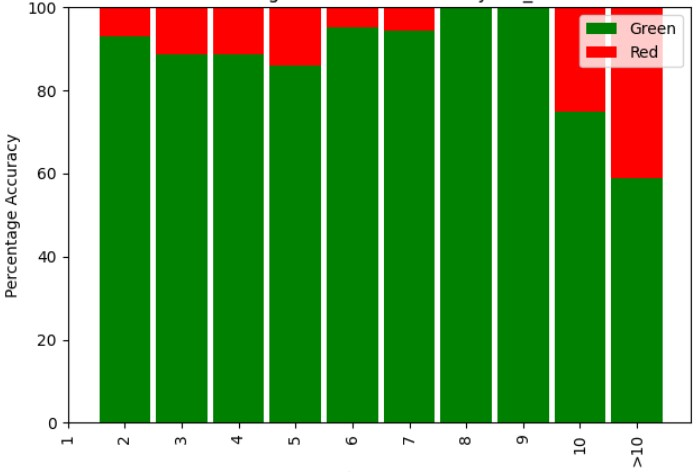
\includegraphics[scale=0.5]{random.jpg} 
\caption{Accuracy vs Sentence Count : subtask-1b3 using mdeberta}
\label{fig.1}
\end{center}
\end{figure}

A different method of evaluation where class 3 is weighed more then others , followed by 2, 1 and 0 might be a better approach as accurately detecting high risk texts should have more importance than whether or not low risk text were detected. Also due to time and cost limitations all approaches haven't been tested which include using an ensemble of above mentioned approaches where keyword-based filtering resulted in near perfect recall scores. This along with one of the transformers or LLM approaches might yield better results. Despite having no context or information regarding the texts, the results appeared quite good. But, it is very likely that with context and other details even better results can be obtained.

Due to the page limitations, some of the omitted information, more plots, prompts used, hyperparameter space explored, and other information along with the code is added in the Appendix.

%placeholder. \footnote{Footnotes should be in  9 pt, and appear at the bottom of the same page as their corresponding number. Footnotes should also be separated from the rest of the text by a 5 cm long horizontal line.}
%All figures should be centred and clearly distinguishable. They should never be drawn by hand, and the lines must be very dark in order to ensure a high-quality printed version. Figures should be numbered in the text, and have a caption in  10 pt underneath. A space must be left between each figure and its respective caption. 
%\begin{figure}[!ht]
%\begin{center}
%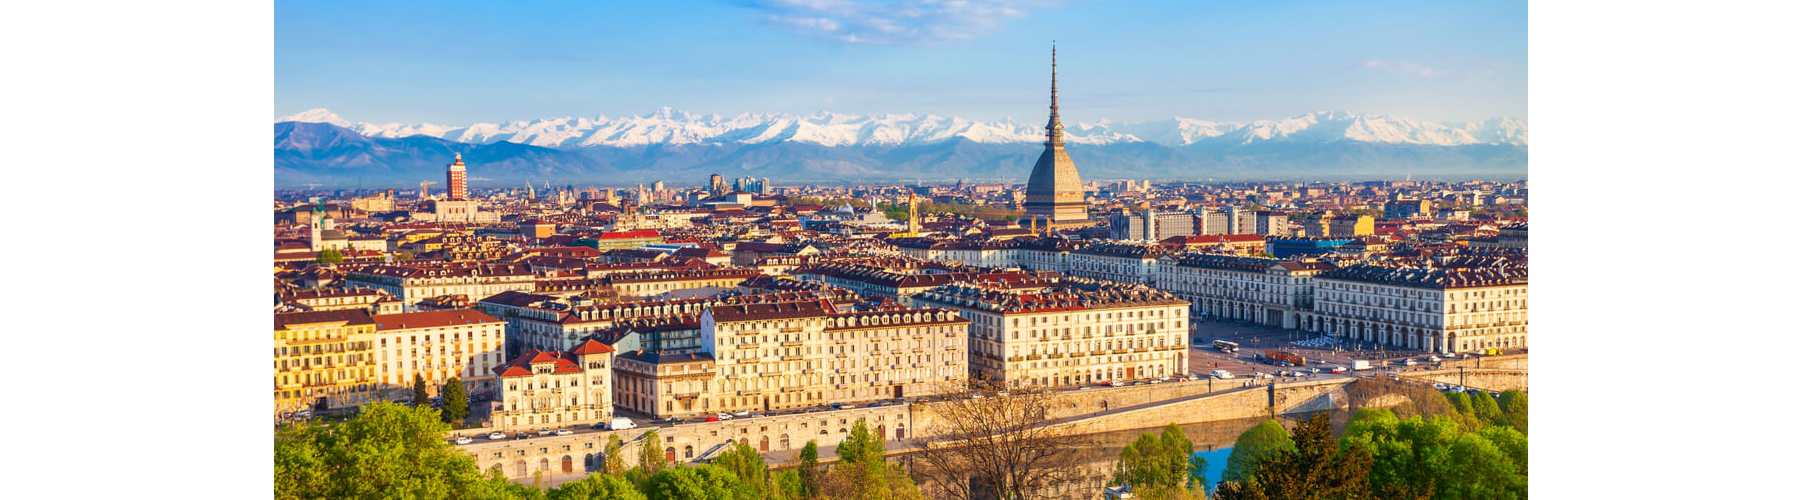
\includegraphics[scale=0.5]{turin2024-banner.jpg} 
%\caption{The caption of the figure.}
%\label{fig.1}
%\end{center}
%\end{figure}
%Figure and caption should always appear together on the same page. Large figures can be centered, using a full page.
%\section{Optional Supplementary Materials}
%Footnotes are indicated within the text by a number in superscript\footnote{Footnotes should be in  9 pt, and appear at the bottom of the same page as their corresponding number. Footnotes should also be separated from the rest of the text by a 5 cm long horizontal line.}.
%Appendices or supplementary material (software and data) will be allowed ONLY in the final, camera-ready version, but not during submission, as papers should be reviewed without the need to refer to any supplementary materials.
%We encourage the submission of these supplementary materials to improve the reproducibility of results and to enable authors to provide additional information that does not fit in the paper. For example, preprocessing decisions, model parameters, feature templates, lengthy proofs or derivations, pseudocode, sample system inputs/outputs, and other details necessary for the exact replication of the work described in the paper can be put into the appendix. However, the paper submissions must remain fully self-contained, as these supplementary materials are optional, and reviewers are not even asked to review or download them. If the pseudo-code or derivations, or model specifications are an essential part of the contribution, or if they are important for the reviewers to assess the technical correctness of the work, they should be a part of the main paper and not appear in the appendix.

%\subsection{Appendices}
%Appendices are material that can be read and include lemmas, formulas, proofs, and tables that are not critical to the reading and understanding of the paper, as in \href{https://acl-org.github.io/ACLPUB/formatting.html#appendices}{*ACLPUB}. It is  highly recommended that the appendices should come after the references; the main text and appendices should be contained in a `single' manuscript file, without being separately maintained. Letter them in sequence and provide an informative title: \textit{Appendix A. Title of Appendix}

%\subsection{Extra space for ethical considerations and limitations}
%Please note that extra space is allowed after the 8th page (4th page for short papers) for an ethics/broader impact statement and a discussion of limitations. At submission time, if you need extra space for these sections, it should be placed after the conclusion so that it is possible to rapidly check that the rest of the paper still fits in 8 pages (4 pages for short papers). Ethical considerations sections, limitations, acknowledgments, and references do not count against these limits. For camera-ready versions, nine pages of content will be allowed for long (5 for short) papers.

\label{Appendix}

\nocite{*}
\section{Bibliographical References}\label{sec:reference}
\bibliographystyle{lrec-coling2024-natbib}
\bibliography{lrec-coling2024-example}
%\section{Language Resource References}
\label{lr:ref}
\bibliographystylelanguageresource{lrec-coling2024-natbib}
\bibliographylanguageresource{languageresource}

\end{document}
%%% Local Variables:
%%% mode: latex
%%% TeX-master: t
%%% End: